\documentclass{chi-ext}

\copyrightinfo{
  Copyright is held by the author/owner(s).\\
  \emph{CHI'12}, May 5--10, 2012, Austin, Texas, USA.\\
  ACM 978-1-4503-1016-1/12/05.\\
}

\title{Sketch It, Make It: Sketching precise drawings for laser cutting}

\numberofauthors{4}

\author{
  \alignauthor{
  	\textbf{Gabe Johnson}\\
  	\affaddr{Carnegie Mellon University}\\
  	\affaddr{Pittsburgh PA}\\
  	\email{johnsogg@cmu.edu}\\
  }\alignauthor{
  	\textbf{Mark D. Gross}\\
  	\affaddr{Carnegie Mellon University}\\
  	\affaddr{Pittsburgh PA}\\
  	\email{mdgross@cmu.edu}\\
  }\\
  \\
  \\
  \alignauthor{
  	\textbf{Ellen Yi-Luen Do}\\
  	\affaddr{Georgia Inst. of Technology}\\
  	\affaddr{Atlanta GA}\\
  	\email{ellendo@gatech.edu}\\
  }\alignauthor{
  	\textbf{Jason I. Hong}\\
  	\affaddr{Carnegie Mellon University}\\
  	\affaddr{Pittsburgh PA}\\
  	\email{jasonh@cs.cmu.edu}\\
  }\\
}

\teaser{
  \centering
  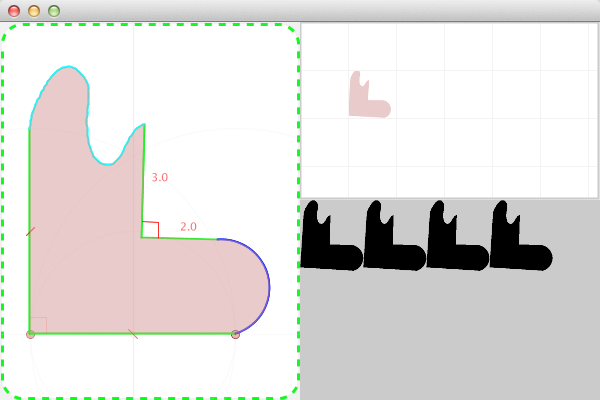
\includegraphics[width=0.87\columnwidth]{img/skruifab-full.png}
  \caption{SIMI enables users to quickly create precise vector
    drawings like this using sketch-based interaction.}
  \label{fig:sample}
}

% Paper metadata (use plain text, for PDF inclusion and later
% re-using, if desired)
\def\plaintitle{Sketch It, Make It} 

\def\plainauthor{Gabe Johnson}

\def\plainkeywords{Sketching, Design, Constraints}

\def\plaingeneralterms{Sketching, Design, Constraints}

\hypersetup{
  % Your metadata go here
  pdftitle={\plaintitle},
  pdfauthor={\plainauthor},  
  pdfkeywords={\plainkeywords},
  pdfsubject={\plaingeneralterms},
  % Quick access to color overriding:
  citecolor=black,
  linkcolor=black,
  menucolor=black,
  urlcolor=black,
}

\usepackage{graphicx}   % for EPS use the graphics package instead
\usepackage{balance}    % useful for balancing the last columns
\usepackage{bibspacing} % save vertical space in references

% ----------------------------------------------------------------------

\begin{document}

\maketitle

\begin{abstract}
Sketch It, Make It (SIMI) is a modeling tool that enables non-experts
to design items for fabrication with laser cutters. SIMI recognizes
rough, freehand input as a user iteratively edits a structured vector
drawing. The tool combines the strengths of sketch-based interaction
with the power of constraint-based modeling. Several interaction
techniques are combined to present a coherent system that makes it
easier to make precise designs for laser cutters.
\end{abstract}

\keywords{\plainkeywords}
% Get CHI keywords and put them here.
\category{I.3.5}{Computational Geometry and Object Modeling}{Modeling packages}


% ======================================================================
\section{Introduction}
% ======================================================================


Rapid fabrication machines such as laser cutters and 3D printers allow
people to make things that would otherwise be too difficult or time
consuming to build. Such machines are becoming more common as their
quality improves and their cost declines. Today's design/build process
typically begins with sketching on paper followed by a session with a
computer tool, and eventually, the fabrication machinery is set to
work.

\begin{figure}
\hspace*{-0.2\columnwidth}% displace figure
\parbox{\columnwidth}{
  \begin{center}
  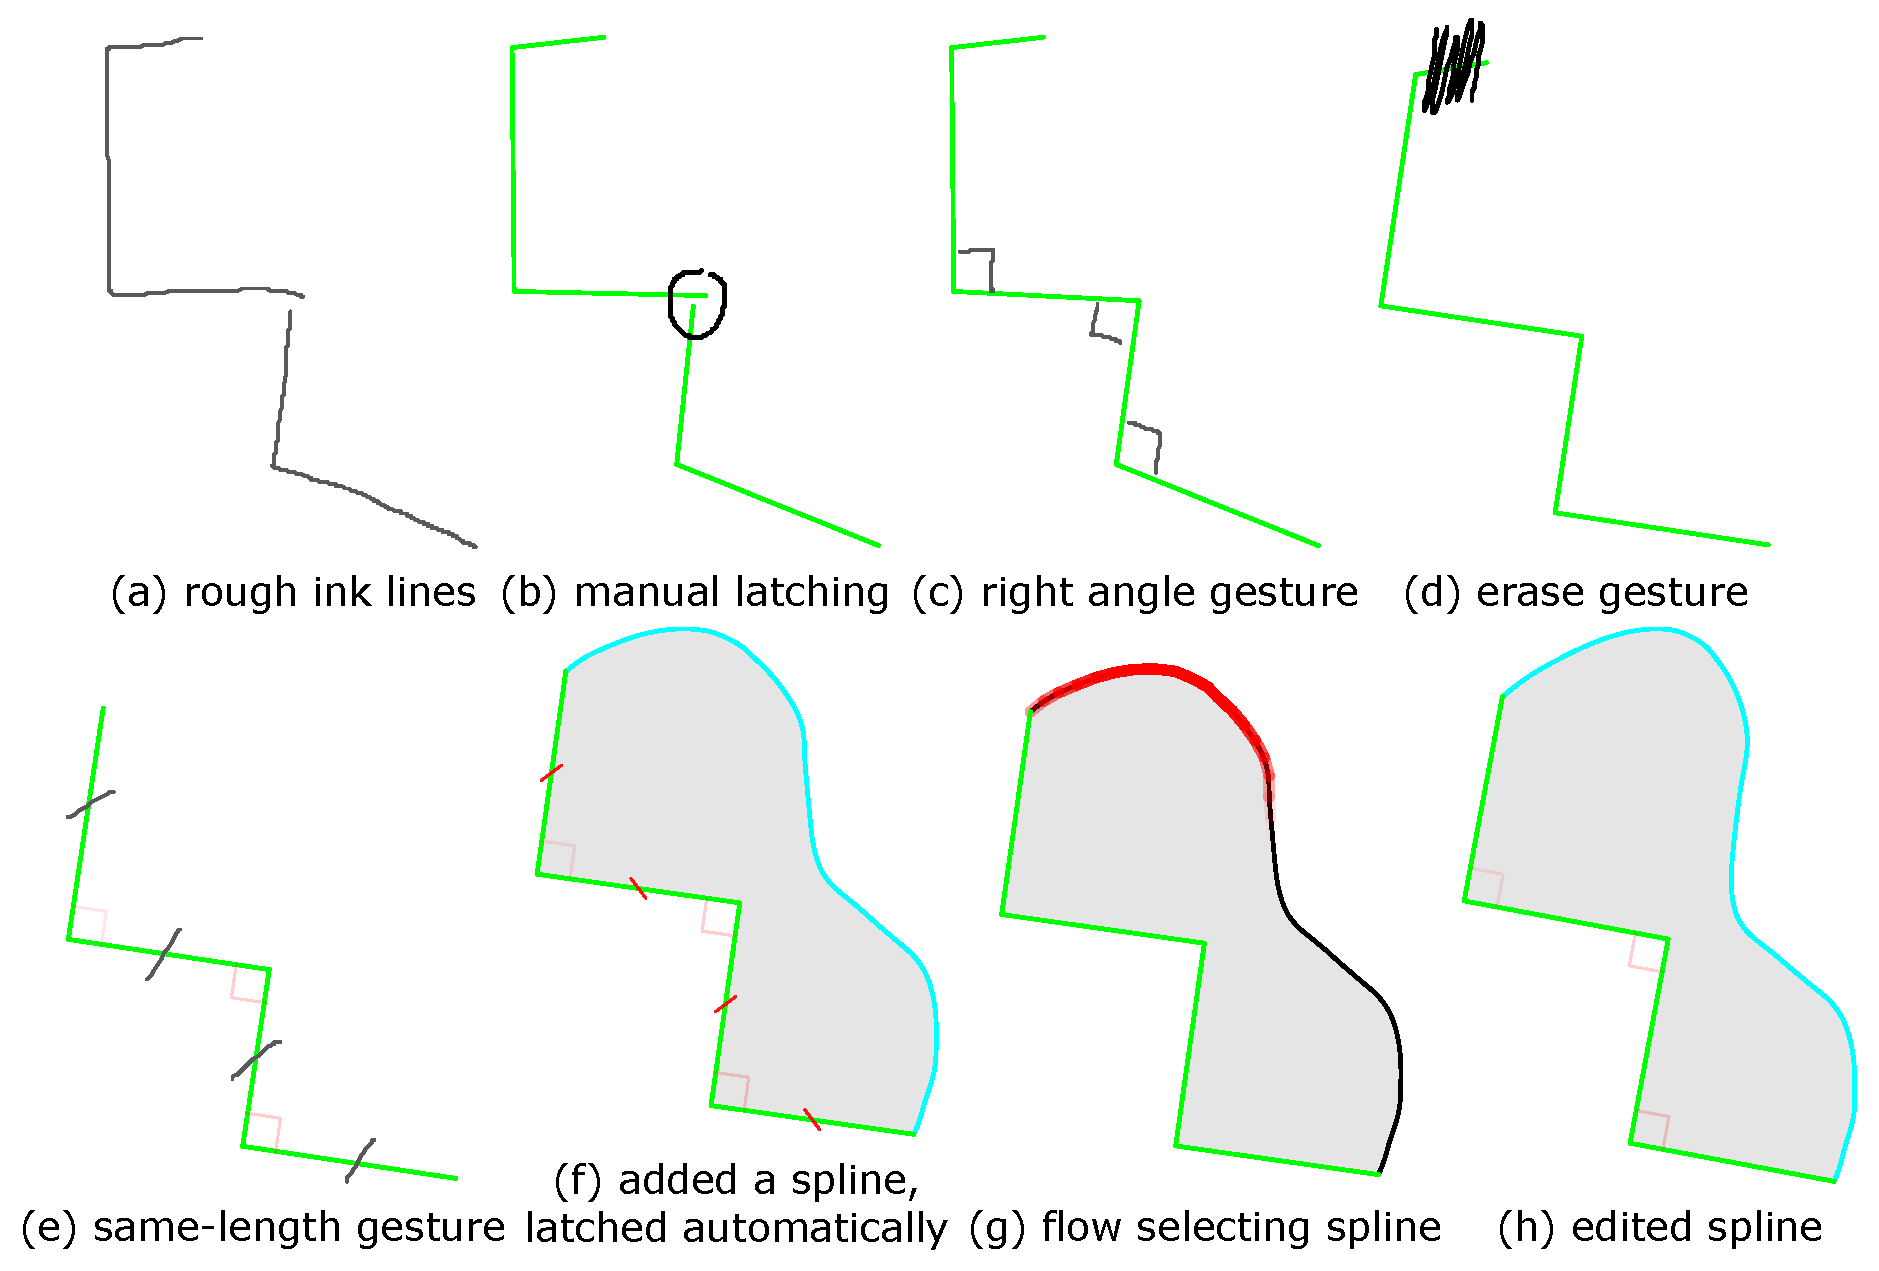
\includegraphics[width=1.2\columnwidth]{img/example-2.pdf}
  \caption{Several sketch interaction techniques for creating and
    editing structured diagrams.}
  \label{fig:bigexample}
  \end{center}  
}
\end{figure}

Unfortunately, people often have difficulty using modeling software
when designing for these machines. The system described in this paper
aims to make it easier and faster for hobbyists and amateurs to move
from idea to specification. Observing that freehand drawing is a
common way to easily give form to ideas, we use this as a starting
point for our design tool.

% =============================================================================
\section{Sketch It, Make It (SIMI)}
% =============================================================================

SIMI presents a set of mutually cohesive sketch-based interaction
techniques for modeling items that will be produced on a laser
cutter. The guiding heuristic for developing these techniques is that
the user should never need to set down the pen. Input is provided
entirely with a stylus and optionally a single button used with the
non-dominant hand.

Many techniques demonstrated in SIMI are inspired by other
sketch-based tools such as ParSketch~\cite{naya-parsketch}, and
Lineogrammer~\cite{zeleznik-lineogrammer}, and
Pegasus~\cite{igarashi-pegasus}. Like SIMI, those systems supported
users to iteratively build structured 2D models using sketch input.

The focus of this work is to produce a useful and usable sketch-based
design tool for the domain of laser cutting. The main challenge in
achieving this was the lack of a set of interaction sketch-based
techniques that work in harmony. Prior work has focused largely on
individual techniques that clearly map problems to solutions. In
contrast, our system address the challenge of developing a system that
integrates many experimental interaction techniques into a coherent
whole.

The system collects rough pen input and invokes recognition after
either a timeout is reached (we use 900ms), or when the user presses
the offhand button. The first two panes of Figure~\ref{fig:bigexample}
illustrate this. When recognition is invoked, SIMI attempts to
interpret the designer's intention by analyzing the most recent
ink. SIMI works best when the recognizer has only a small number of
strokes (e.g. 6 or fewer) to work with. The intended interaction is a
rhythmic cycle where the user draws a few strokes, invokes recognition,
and continues.

The shape made in Figure~\ref{fig:bigexample} is composed of straight
lines and a free-form spline. Closed shapes are shaded slightly,
indicating complete stencils ready for laser cutting. Stencil
interiors are allowed to have holes (e.g. to accept screws).

SIMI first segments input into primitive parts: dots, lines,
elliptical arcs, and splines. We use a segmentation and corner finding
strategy based on MergeCF~\cite{wolin-smr}. Elliptical segments may be
at any angle, and are found with the least-squares method described by
Fitzgibbon \textit{et. al}~\cite{fitzgibbon-ellipse-fitting}.

SIMI also recognizes commands that manipulate existing geometry
(illustrated in Figure~\ref{fig:bigexample}). All commands are
context-sensitive. For example, SIMI recognizes a right angle when it
identifies a half-square symbol near the intersection of two line
segments.

SIMI does not have persistent modes. Rather than requiring users to
invoke modal tools such as line, select, erase, and so on, SIMI
deduces the user's intention via recognition.

Most commands are recognized after the timeout or when the button is
pressed. But some frequently used commands (erase, latch) are
immediate, and are triggered by gestures that are unlikely to be
confused with other ink.

\subsection{Latching}

\marginpar{
\begin{figure}
  \begin{center}
  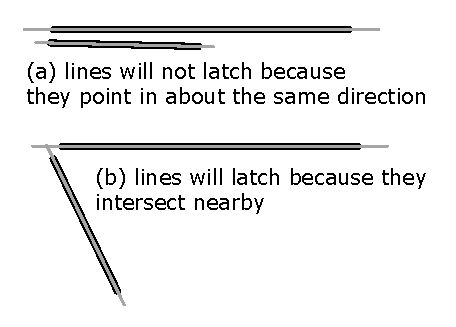
\includegraphics[width=\marginparwidth]{img/latch.pdf}
  \caption{Automatic latching depends on endpoint position, relative
    angle, and segment lengths.}
  \label{fig:latch}
  \end{center}  
\end{figure}
}

\marginpar{
\begin{figure}
  \begin{center}
  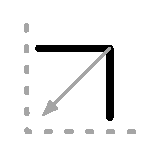
\includegraphics[width=\marginparwidth]{img/right-angle.pdf}
  \caption{Right angle gesture (dark) will be applied if (and only if)
    it is near a junction resembling the light, dashed lines.}
  \label{fig:right-angle}
  \end{center}  
\end{figure}
}

SIMI supports latching endpoints of two nearby segments. The system
automatically latches endpoints just after recognizing new line
work. For each new segment, SIMI identifies all others with nearby
endpoints and forms candidate pairs. For each pair, segment extensions
are extrapolated based on the segment's type (e.g. line or arc) (shown
in light, thin lines in Figure~\ref{fig:latch}. The extensions are
10\% of the total line length, or 10 pixels, whichever is larger. If
the two extended segments intersect, SIMI latches them.

SIMI lets users quickly merge nearby points manually. This technique
was inspired by the lasso gesture in Bae's EverybodyLovesSketch
system~\cite{bae-everybody}. To merge nearby endpoints, the user draws
a small circle around them.

\subsection{Scribble Erase}

The designer removes items by scratching them out. Line work,
constraints, and unrecognized ink can all be erased. The scribble
recognizer executes as the stroke is made. It recognizes scribbles by
sampling the most recent pen input and looks for abrupt changes in
direction. When enough of these abrupt changes are found in a short
time period it triggers an erase and signals this with visual
feedback.

Next, suitable targets are sought. If only one object is underneath
the scribble, it is removed. If the gesture covers several objects,
SIMI compares the scribble's area with each object's area. When more
than 60\% of an object is under scribble, it is erased. If no objects
match that rule, then the one with the most area under the scribble is
removed. This makes it possible to accurately remove small items that
are near larger ones.

\subsection{Right Angle}

Right angles are frequently needed in laser-cut items. To make
perpendicular, the user draws two short lines that meet, in the
conventional `right angle' symbol. If this symbol appears near a
junction that is 90$^{\circ}$ (\pm15$^{\circ}$), the segments
composing that junction will be constrained to meet at exactly a right
angle, as shown in Figure~\ref{fig:right-angle}.

\subsection{Same Length}

Users may instruct SIMI to make several segments the same length by
drawing hashes on them. This can be done in one batch (as in
Figure~\ref{fig:bigexample}), or in several by hashing a constrained
segment and additional unconstrained segments. The constraint engine
uses the mean length as the target value.

\subsection{Flow Selection}

SIMI lets users edit the shape of curves by using flow
selection~\cite{johnson-flow-selection}. The user briefly dwells the
pen near a spline, growing the selection area. Then, without lifting
the stylus up, the designer moves it to reshape the selected region.

\section{Constraint Engine}

Most of SIMI's commands relate to establishing geometric rules
(constraints), such as ``make this line perpendicular to that line'',
``make these segments the same length''. SIMI's custom-built 2D engine
is a numeric, iterative solver. The engine incrementally moves
vertices and other objects until all constraints are satisfied, or
until it determines it can not find a solution. The details of the
constraint solver are beyond the scope of this paper.

\section{Future Work}

This work borrows conventions from disciplines such as mechanical
engineering and architecture. Techniques like hatching (e.g. to
indicate similar regions) deserve consideration. We are currently
exploring ways to use temporary guides (e.g. straight edges, French
curves) to aid drawing.

SIMI should also support zooming. Laser-cut items often contain small
regions that require great detail that are difficult to draw without
zooming in. The system does not yet recognize character input for
adding dimensions to angles and lengths. For now we ``cheat'' by
allowing keyboard input.

In the near future we will begin testing SIMI with students who
regularly use laser cutters. This will help guide development.

\balance
\bibliographystyle{acm-sigchi}
\bibliography{simi}

\end{document}

